\documentclass[paperwidth=46.8in,paperheight=26.3in,fontscale=0.35]{baposter}

\usepackage[vlined]{algorithm2e}
\usepackage{times}
\usepackage{calc}
\usepackage{url}
\usepackage{graphicx}
\usepackage{amsmath}
\usepackage{amssymb}
\usepackage{relsize}
\usepackage{multirow}
\usepackage{booktabs}

\usepackage{graphicx}
\usepackage{multicol}
\usepackage[T1]{fontenc}
\usepackage{ae}
\usepackage{enumitem}


\usepackage{colortbl}
\usepackage{xcolor}
%\usepackage{gensymb} % for \degree

%%%
\usepackage{subfigure}
\usepackage[T1]{fontenc}
\usepackage{latexsym,amsmath,xcolor,multicol,booktabs,calligra}
\usepackage{graphicx,pstricks,listings,stackengine}
\usepackage{bm}
\usepackage{tikz}

% define colors
\xdefinecolor{comsoc}{RGB}{0,86,125}
\xdefinecolor{icc}{RGB}{0,174,239}

% custemize itemize and enumerate
\setlist[itemize]{leftmargin=*,nosep}
    \setlength{\columnsep}{0.7em}
    \setlength{\columnseprule}{0mm}
\newcommand*\circled[1]{\tikz[baseline=(char.base)]{%
    \node[shape=circle,fill=comsoc,draw,inner sep=0pt] (char) {{\scriptsize{#1}}};}}
\setlist[enumerate]{leftmargin=*,nosep,label=\protect\circled{\color{white}\arabic*}}
    \setlength{\columnsep}{1.0em}
    \setlength{\columnseprule}{0mm}

% %%%%%%%%%%%%%%%%%%%%%%%%%%%%%%%%%%%%%%%%%%%%%%%%%%%%%%%%%%%%%%%%%%%%%%%%%%%%%%%%
% % Save space in lists. Use this after the opening of the list
% %%%%%%%%%%%%%%%%%%%%%%%%%%%%%%%%%%%%%%%%%%%%%%%%%%%%%%%%%%%%%%%%%%%%%%%%%%%%%%%%
\setlength{\itemsep}{0pt}
\setlength{\itemsep}{0pt}
\setlength{\parskip}{0pt}
\setlength{\parsep}{0pt}

\setlength{\abovecaptionskip}{0.cm}
\setlength{\belowcaptionskip}{0.cm}

\setlength{\abovedisplayskip}{-10pt}
\setlength{\belowdisplayskip}{-10pt}
\setlength{\abovedisplayshortskip}{-10pt}
\setlength{\belowdisplayshortskip}{-10pt}

\renewcommand{\rmdefault}{ptm} % Arial
\renewcommand{\sfdefault}{ptm} % Arial

\newcommand{\vn}{\boldsymbol{n}}
\newcommand{\vl}{\boldsymbol{l}}
\newcommand{\vM}{\mathbf{M}}
\newcommand{\vN}{\mathbf{N}}
\newcommand{\vL}{\mathbf{L}}
%%%%%%%%%%%%%%%%%%%%%%%%%%%%%%%%%%%%%%%%%%%%%%%%%%%%%%%%%%%%%%%%%%%%%%%%%%%%%
%% Begin of Document
%%%%%%%%%%%%%%%%%%%%%%%%%%%%%%%%%%%%%%%%%%%%%%%%%%%%%%%%%%%%%%%%%%%%%%%%%%%%%
\begin{document}
%%%%%%%%%%%%%%%%%%%%%%%%%%%%%%%%%%%%%%%%%%%%%%%%%%%%%%%%%%%%%%%%%%%%%%%%%%%%%
%% Here starts the poster
%%---------------------------------------------------------------------------
%% Format it to your taste with the options
%%%%%%%%%%%%%%%%%%%%%%%%%%%%%%%%%%%%%%%%%%%%%%%%%%%%%%%%%%%%%%%%%%%%%%%%%%%%%
\begin{poster}{
    % Poster Environment Options
    grid=false,
    columns=4,
    colspacing=0.7em,
    headerheight=0.12\textheight,
    background=none,
    bgColorOne=white,
    bgColorTwo=white,
    eyecatcher=true,
    % Posterbox Environment Options
    borderColor=comsoc,
    headerColorOne=comsoc,
    headerColorTwo=comsoc,
    textborder=faded,
    headerborder=open,
    headershape=roundedright,
    headershade=plain
    }
    % University logo
    {
    \makebox[0.005\textwidth]{}
    \raisebox{0.07\height}{
\includegraphics[width=0.045\linewidth]{logo/SUSTech_logo.png}}
    \makebox[0.005\textwidth]{}
    \raisebox{0.07\height}{
\includegraphics[width=0.045\linewidth]{logo/HKU_logo.png}}
    \makebox[0.005\textwidth]{}
    \raisebox{0.07\height}{
\includegraphics[width=0.045\linewidth]{logo/USTC_logo.png}}
    }
    % Title
    {
    \sc\Huge\bf Predictive Resource Allocation in mmWave Systems with Rotation Detection
    }
    % Authors
    {
    \vspace{0.3em}
    {Yifei~Sun{\textsuperscript\textdagger}{\textsuperscript\textdaggerdbl},
    ~Bojie~Lv{\textsuperscript\textdagger},
    ~Rui~Wang{\textsuperscript\textdagger},
    ~Haisheng~Tan{\textsuperscript\textsection},
    ~and~Francis~C.~M.~Lau{\textsuperscript\textdaggerdbl}} \\[0.2em]
    {\Large{\textsuperscript\textdagger}Southern University of Science and Technology,
    ~{\textsuperscript\textdaggerdbl}The University of Hong Kong,
    ~{\textsuperscript\textsection}University of Science and Technology of China}
    }
    % Eye Catcher
    {
    \begin{tabular}{c}
        \raisebox{-0.0\height}{
\includegraphics[width=0.12\linewidth]{logo/ICC2023_logo.png}} \\
        \raisebox{-0.0\height}{
\includegraphics[width=0.12\linewidth]{logo/ICC2023_info.png}}
    \end{tabular}
    }

    %%%%%%%%%%%%%%%%%%%%%%%%%%%%%%%%%%%%%%%%%%%%%%%%%%%%%%%%%%%%%%%%%%%%%%%%%%%%%%
    %%% Now define the boxes that make up the poster
    %%%---------------------------------------------------------------------------
    %%% Each box has a name and can be placed absolutely or relatively.
    %%% The only inconvenience is that you can only specify a relative position 
    %%% towards an already declared box. So if you have a box attached to the 
    %%% bottom, one to the top and a third one which should be inbetween, you 
    %%% have to specify the top and bottom boxes before you specify the middle 
    %%% box.
    %%%%%%%%%%%%%%%%%%%%%%%%%%%%%%%%%%%%%%%%%%%%%%%%%%%%%%%%%%%%%%%%%%%%%%%%%%%%%%

    %%%%%%%%%%%%%%%%%%%%%%%%%%%%%%%%%%%%%%%%%%%%%%%%%%%%%%%%%%%%%%%%%%%%%%%%%%%%%%
    \headerbox{\bf\color{white} Introduction}{name=introduction,column=0,row=0,span=2}{
        \textbf{\color{icc}Motivation:}
        \begin{enumerate}
            \item UE rotation may cause significant SNR fluctuation, thus QoS degradation, in mmWave systems.
            \item UE-embedded motion sensors enable predictive SNR fluctuation with statistical channel model.
            \item This raises a new design issue of large-time-scale scheduling with non-stationary but predictable channel statistics.
        \end{enumerate}
        \begin{minipage}{0.55\linewidth}
            \begin{center}
                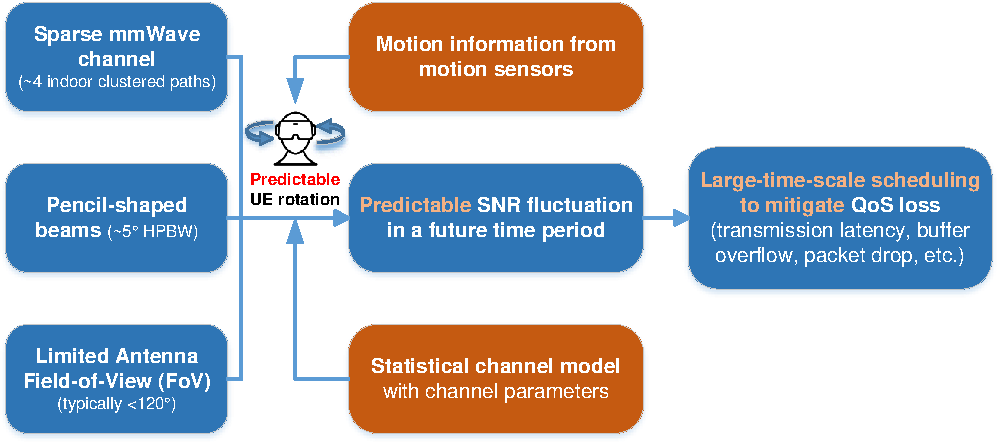
\includegraphics[width=\textwidth]{fig/pre_motivation_scheme_predict_v1_1.pdf}
            \end{center}
        \end{minipage}
        \hfill
        \begin{minipage}{0.43\linewidth}
            \begin{center}
                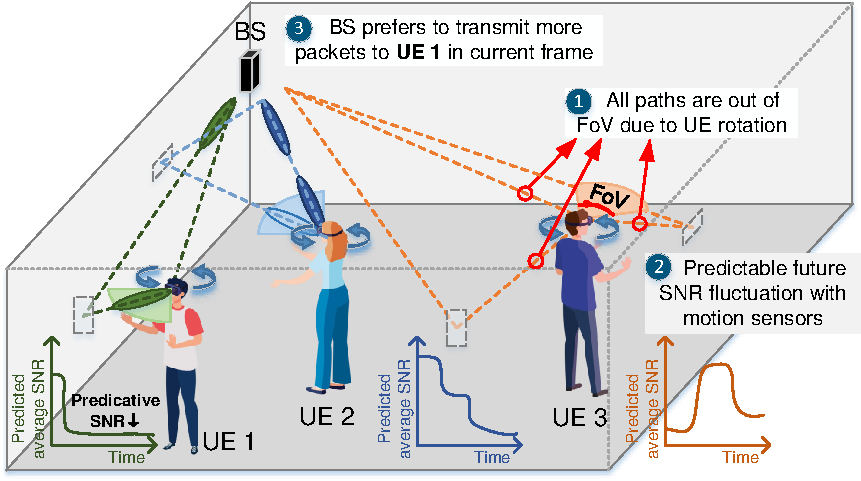
\includegraphics[width=\textwidth]{fig/pre_motivation_scenario_predict_v1_2.pdf}
            \end{center}
        \end{minipage}
    }

    \headerbox{\bf\color{white} System Model}{name=system,column=0,below=introduction,span=2}{
        \begin{minipage}[t]{0.54\linewidth}
            \vspace{0.0em}
            \textbf{\color{icc}Network Description:}
            \begin{itemize}
                \item Downlink transmission with one BS and $K$ rotating UEs.
                \item \textbf{Predictable UE orientation:} UE orientation in future $T$ frames can be predicted by orientation prediction methods (e.g., constant angular velocity).
                \item \textbf{Analog MIMO transceivers:} each with a single RF chain and a limited-FoV ULA.
                \item \textbf{Finite buffer size:} $K$ downlink queues at the BS each with limited buffer size $Q_{\mathrm{max}}$ and \textbf{random arrival}. Buffer overflow will lead to packet drop.
            \end{itemize}
            \textbf{\color{icc}Cluster-based Channel Model:}
            \begin{align*}
                \mathbf{H}_{t,k}
                \!=\!
                \sum_{i=1}^{N_{k}^{\mathrm{cl}}}\!
                \sum_{\ell=1}^{N_{k,i}^{\mathrm{ray}}}\!
                \underbrace{\alpha_{t,k,i,\ell}}_{\textrm{complex gain}}
                \underbrace{\mathbf{a}_{\mathrm{R}}(\!\phi_{t,k,i,\ell}\!)
                \mathbf{a}_{\mathrm{T}}^{\mathsf{H}}(\!\theta_{t,k,i,\ell}\!)}_{\textrm{array responses}}
                \underbrace{\Lambda_{\mathrm{R}}(\!\phi_{t,k,i,\ell}\!)
                    \Lambda_{\mathrm{T}}(\!\theta_{t,k,i,\ell}\!)}_{\textbf{antenna pattens (w/ limited FoV)}}
            \end{align*}
            \textbf{\color{icc}Predictable Average SNR:}
            \begin{itemize}
                \item With pre-learned quasi-static statistical channel parameters, the only non-stationary parameter, \textbf{cluster mean AoA} ${\blue{\bar{\phi}_{t,k,i}}}$ due to UE rotation, can be predicted with constant angular velocity $\omega_{k}$,
                      \begin{align*}
                          \bar{\phi}_{t,k,i}=\bar{\phi}_{1,k,i}+(t-1)\omega_{k}T_{\mathrm{F}}.
                      \end{align*}
                \item Future average SNR can be predicted by
                      \begin{align*}
                          \overline{\textrm{SNR}}_{t,k}
                          =
                          \mathbb{E}_{\mathbf{H}_{t,k}}\frac{P_{t,k}\big|\mathbf{w}_{t,k}^{\mathsf{H}}\mathbf{H}_{t,k}\mathbf{f}_{t,k}\big|^{2}}{N_{0}W}.
                      \end{align*}
            \end{itemize}
        \end{minipage}
        \hfill
        \begin{minipage}[t]{0.44\linewidth}
            \vspace{0.0em}
            \begin{center}
                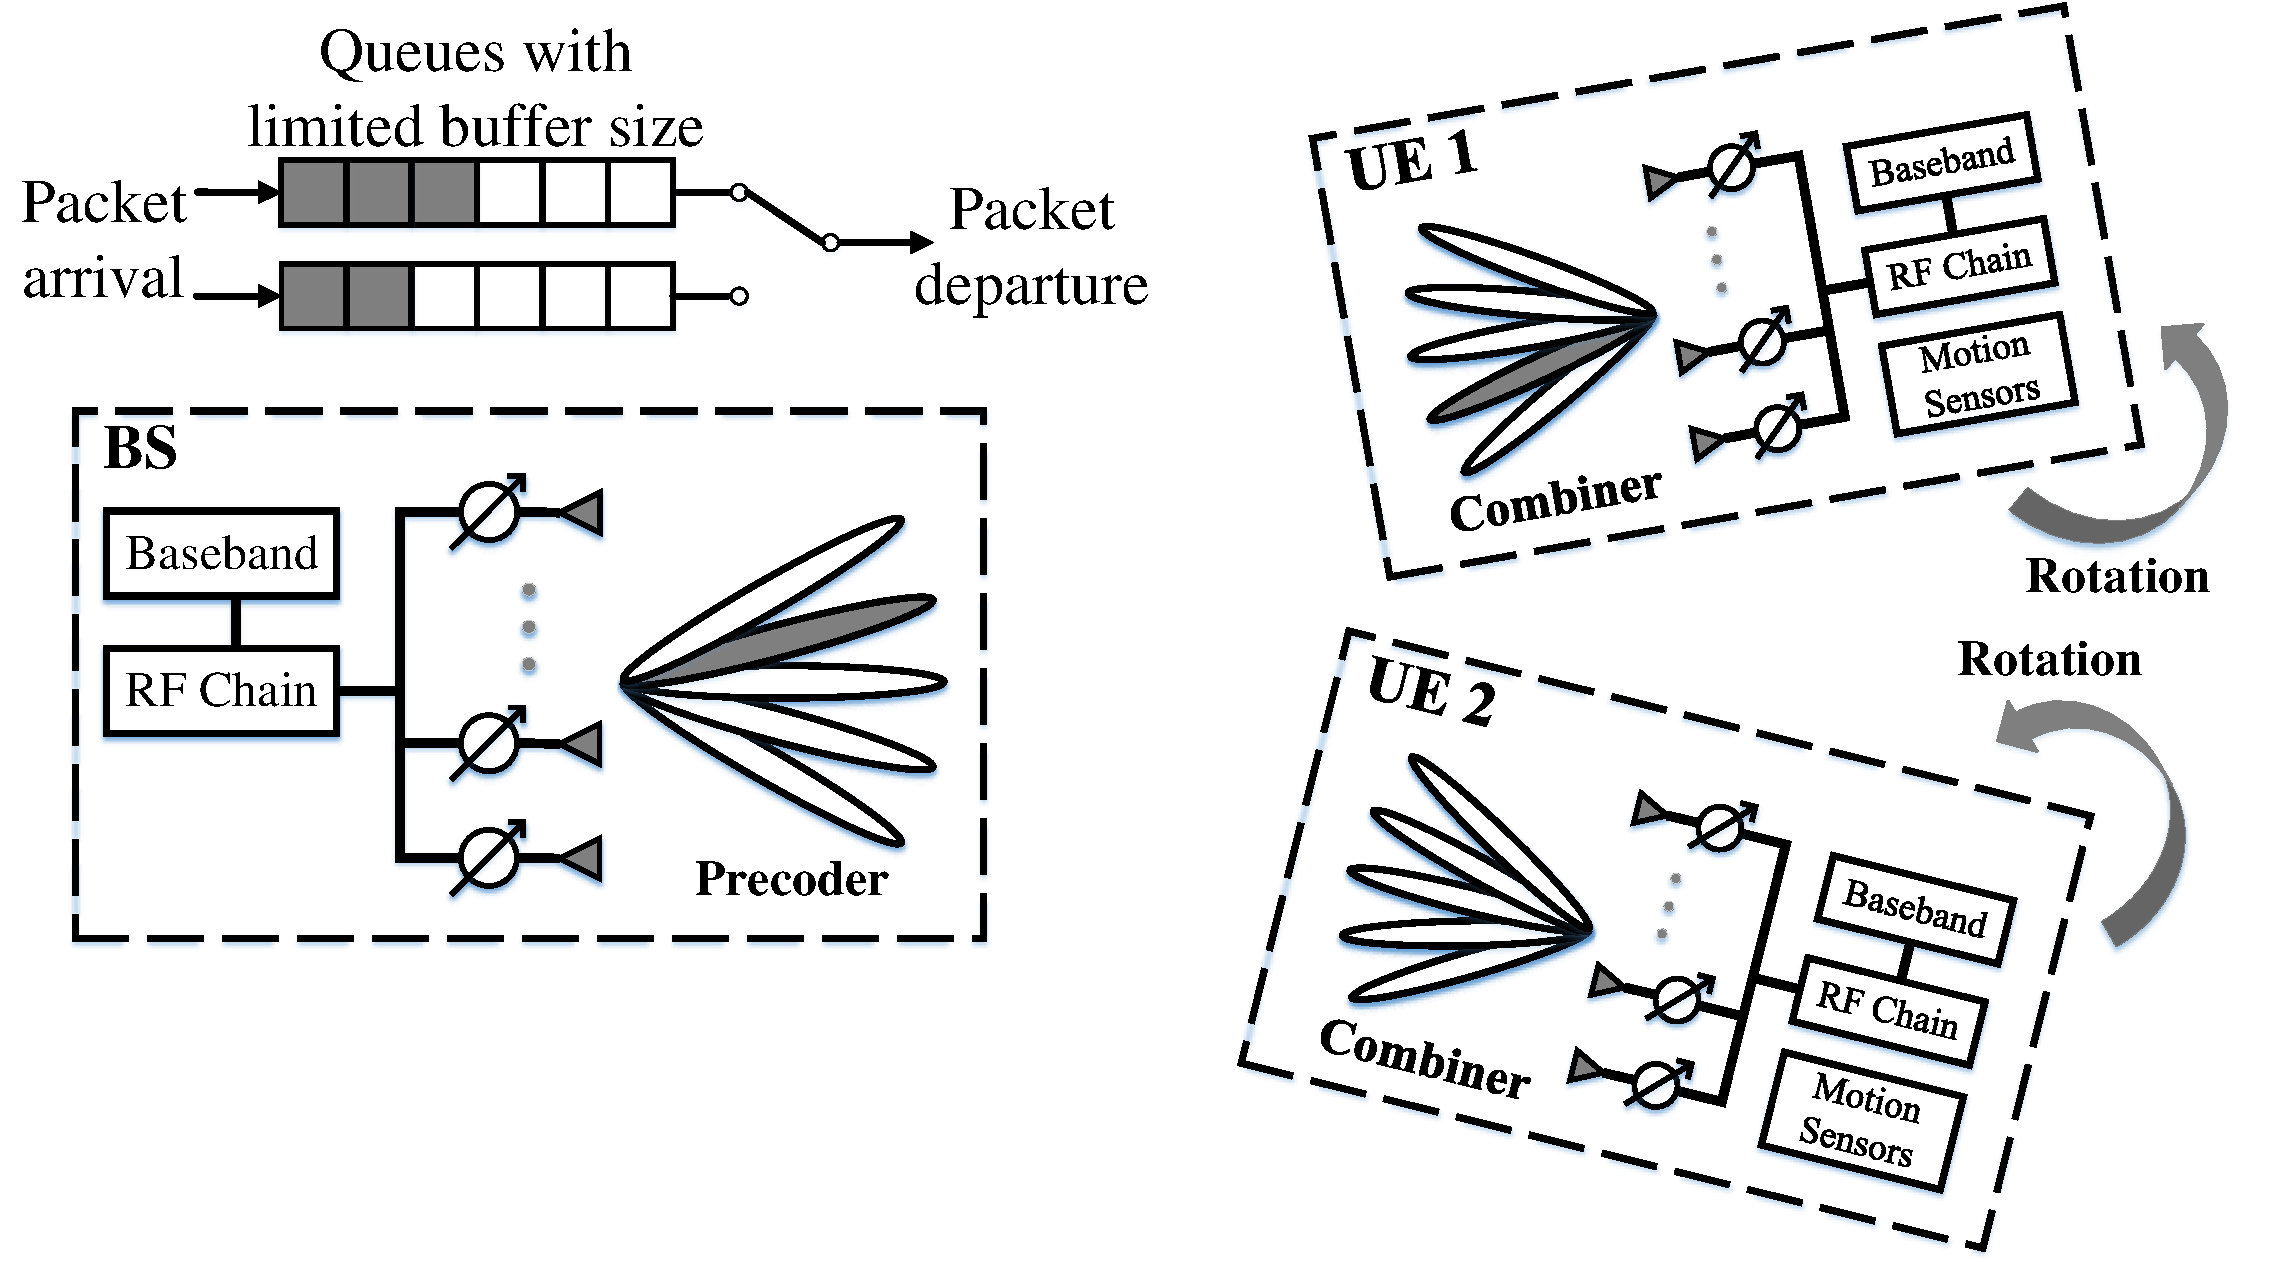
\includegraphics[width=\textwidth]{fig/system_model_v1_4a.pdf}
            \end{center}
            \begin{center}
                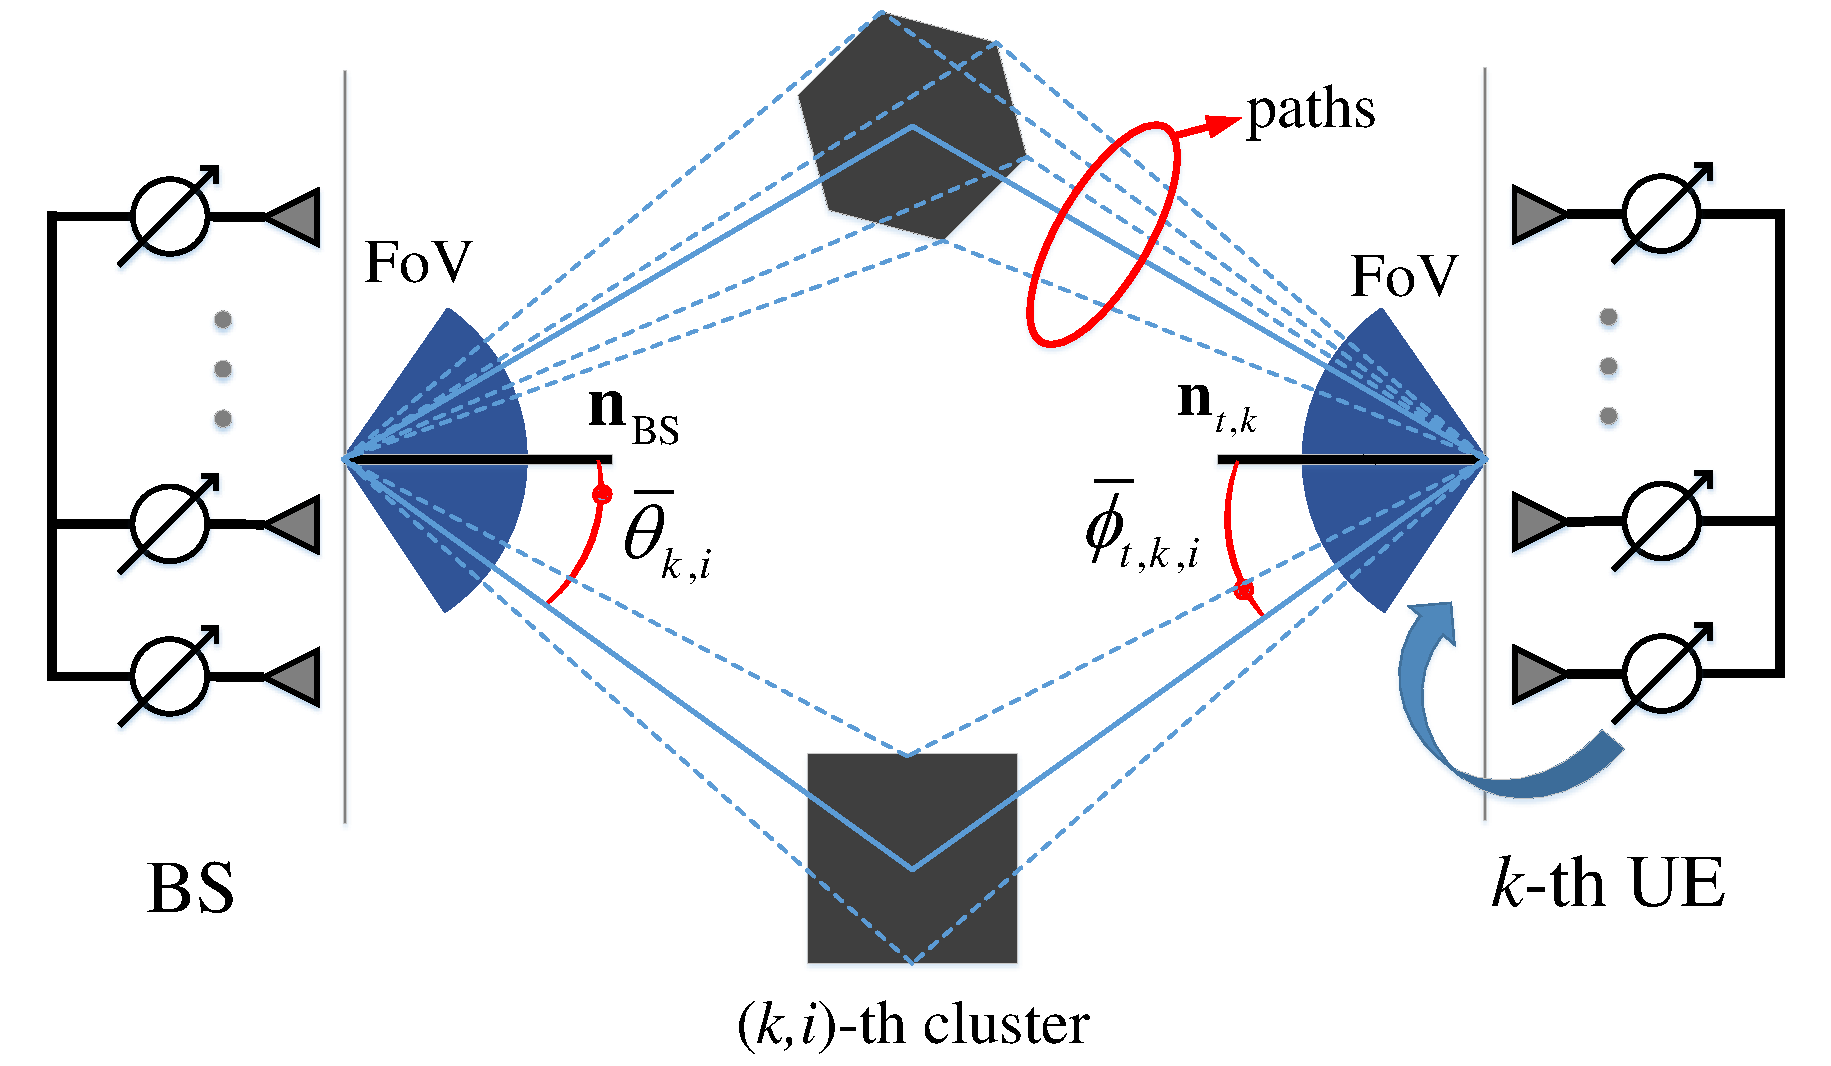
\includegraphics[width=\textwidth]{fig/system_model_v1_4b.pdf}
            \end{center}
        \end{minipage}
    }

    \headerbox{\bf\color{white} Problem Formulation}{name=problem,column=2,row=0,span=1}{
        \textbf{\color{icc}Finite-horizon MDP:}
        \begin{itemize}
            \item \textbf{Finite horizon (stages \#):} because the system can predict UE orientation in $T$ frames (one scheduling period).
                  % \item \textbf{State:} Queue lengths $\mathcal{Q}_{t}$ and baseband channel power gains $\mathcal{Y}_{t}$.
                  % \item \textbf{Action:} UE selection $d_{t}$ and downlink power $P_{t}$.
            \item \textbf{Per-frame cost:}
                  \vspace{-1em}
                  \begin{align*}
                      g_{t}\big(\mathcal{S}_{t},\Omega_{t}(\mathcal{S}_{t})\big)
                      \!\triangleq\!
                      \underbrace{w_{\mathrm{P}}P_{t}}_{\textrm{downlink power}\atop\textrm{consumption}}
                      \!+\!
                      \sum_{k\in\mathcal{K}}\big(\!\underbrace{Q_{t,k}}_{\textrm{queue}\atop\textrm{length}}
                      \!+\!
                      \underbrace{w_{\mathrm{Q}}\mathbb{I}[Q_{t,k}\!=\!{Q}_{\mathrm{max}}]}_{\textrm{packet-drop penalty}}\!\big)
                  \end{align*}
        \end{itemize}
        \begin{center}
            \vspace{-1em}
            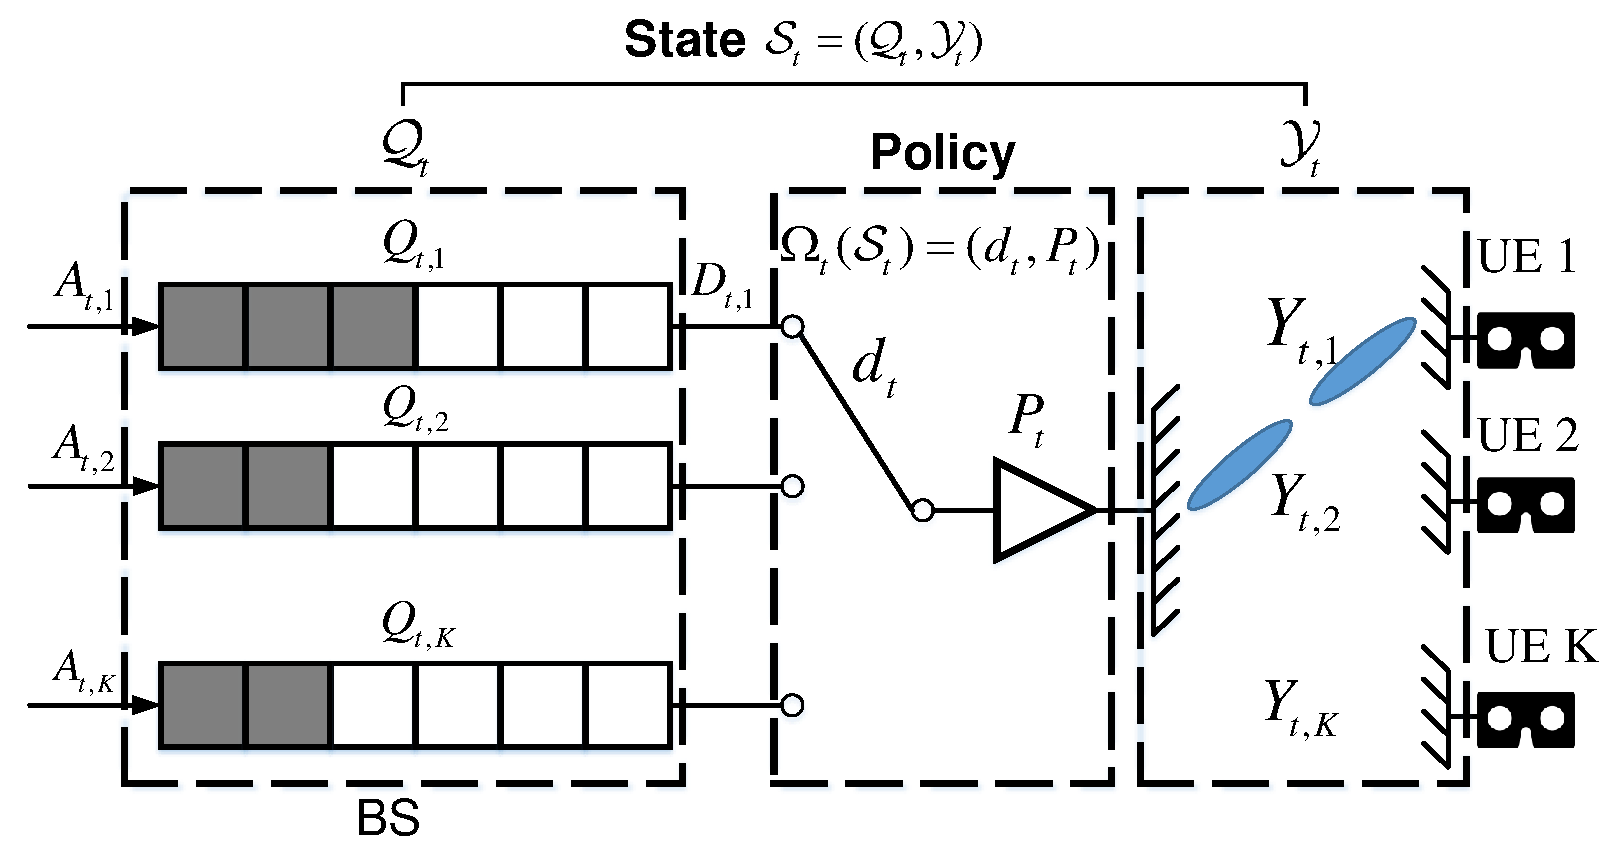
\includegraphics[width=\textwidth]{fig/pre_MDP_problem_formulation_v1_0.pdf}
        \end{center}
        \vspace{-1.5em}
        \textbf{\color{icc}Dynamic Programming Problem:}
        \begin{itemize}
            \item To minimize the weighted sum of downlink energy consumption, queuing delay and packet-drop rate in future $T$ frames.
        \end{itemize}
        \vspace{-1em}
        \begin{align*}
            \bm{\mathsf{P1:}}\ \Omega^{\star}
            \!\triangleq\!
            \{\Omega_{t}^{\star}|\forall t\}
            \!=\!
             &
            \mathop{\arg\min}_{\Omega}\mathbb{E}_{\mathcal{A},\mathcal{Y}}^{\Omega}\big[\sum_{t\!=\!1}^{T}g_{t}\big(\!\mathcal{S}_{t},\Omega_{t}(\!\mathcal{S}_{t}\!)\!\big)\big|\mathcal{S}_{1}\big] \\
             &
            \mathrm{s.t.}\quad 0\leq P_{t}\leq P_{\mathrm{max}},\ \forall t.
        \end{align*}
    }

    \headerbox{\bf\color{white} Proposed Solution}{name=solution,column=3,row=0,span=1}{
        \textbf{\color{icc}Low-complexity Suboptimal Solution Framework:}
        \begin{center}
            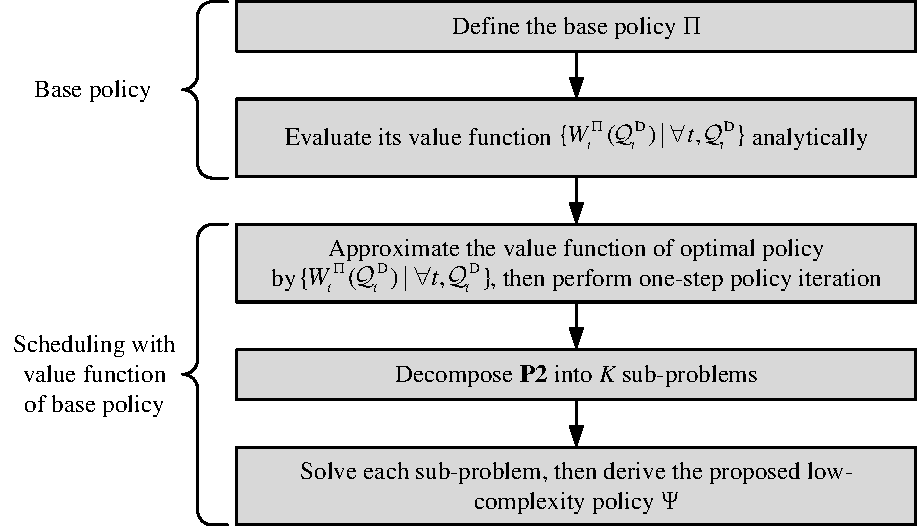
\includegraphics[width=\textwidth]{fig/pre_solution_framework_v1_0.pdf}
        \end{center}
        \begin{itemize}
            \vspace{-1em}
            \item \textbf{Base Policy $\Pi$:} UE selection based on \textit{backpressure algorithm}, and constant downlink transmission power.
            \item \textbf{One-step policy improvement:}
                  \vspace{-1em}
                  \begin{align*}
                      \bm{\mathsf{P2:}} \Psi_{t}(\mathcal{S}_{t})
                      =
                      \mathop{\arg\min}_{\Omega_{t}(\mathcal{S}_{t})}\big\{g_{t}\big(\mathcal{S}_{t},\Omega_{t}(\mathcal{S}_{t})\big)
                      \!+\!
                      W_{t}^{\Pi}\big(\mathcal{Q}_{t}^{\mathrm{D}}(\mathcal{S}_{t},\Omega_{t})\big)\big\},
                  \end{align*}
        \end{itemize}
        \vspace{-1em}
        \textbf{\color{icc}Advantages:}
        \begin{itemize}
            \item \textbf{Low-complexity:} analytical expressed value function of base policy, and one-step value iteration.
            \item \textbf{Offline base policy evaluation} with reduced state space.
            \item \textbf{Distributed online scheduling} with small signaling overhead.
            \item \textbf{Performance Guarantee:} lower bounded by base policy.
        \end{itemize}
    }

    \headerbox{\bf\color{white} Simulation Results}{name=results,column=2,below=problem,span=2}{
        \begin{minipage}[t]{0.27\linewidth}
            \vspace{0.0em}
            \textbf{\color{icc}How it Works: \\an Illustrative Run}
            \begin{itemize}
                \item Instantaneous SNR and queue dynamics of a static UE (k=1) and a rotating UE (k=5).
                \item The proposed scheme can predictively schedule more transmission opportunities to a rotating UE (k=5) about 20 frames before its SNR degrades, so that the future packet drop rate can be significantly reduced.
                \item \textbf{Benchmarks:} \\
                      Dynamic BackPressure (DBP) \\
                      Largest-Rate First (LRF)\\
                      Longest-Queue First (LQF)
            \end{itemize}
        \end{minipage}
        \hfill
        \begin{minipage}[t]{0.48\linewidth}
            \vspace{0.0em}
            \begin{center}
                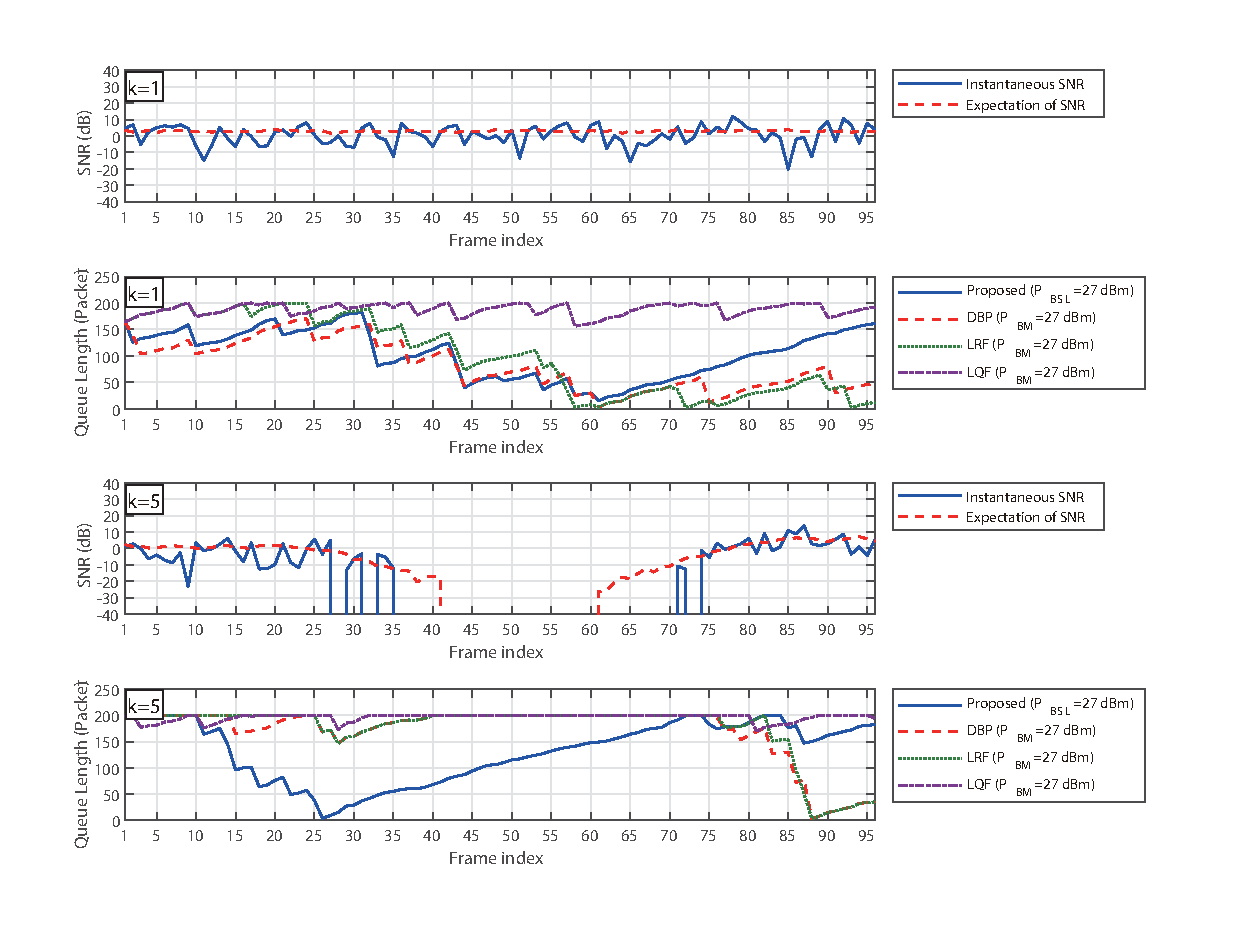
\includegraphics[width=\textwidth]{fig/scenario3_insight_v4.pdf}
            \end{center}
        \end{minipage}
        \hfill
        \begin{minipage}[t]{0.21\linewidth}
            \vspace{0.0em}
            \textbf{\color{icc}CDF of per-frame cost:}
            \begin{center}
                \vspace{-0.8em}
                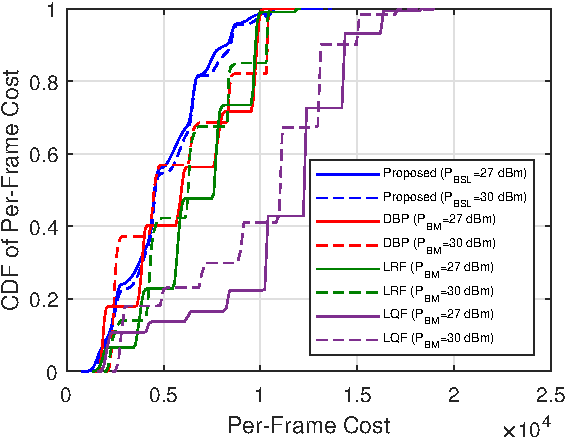
\includegraphics[width=\textwidth]{fig/scenario3_CDF.pdf}
            \end{center}
            \vspace{-1em}
            \textbf{\color{icc}Average component cost:}
            \begin{center}
                \vspace{-0.8em}
                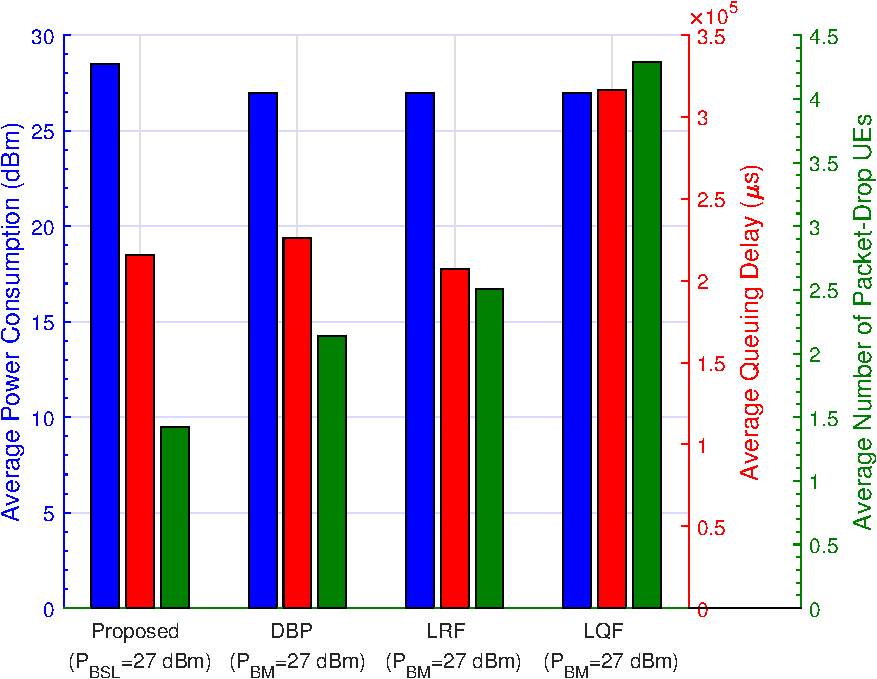
\includegraphics[width=\textwidth]{fig/scenario3_bar27.pdf}
            \end{center}
        \end{minipage}
    }

\end{poster}
\end{document}
